\section{Actividad 02: Creación del primer paquete DTSX} 


1. Abriremos un nuevo Proyecto en nuestro Visual Studio\\
	\begin{center}
	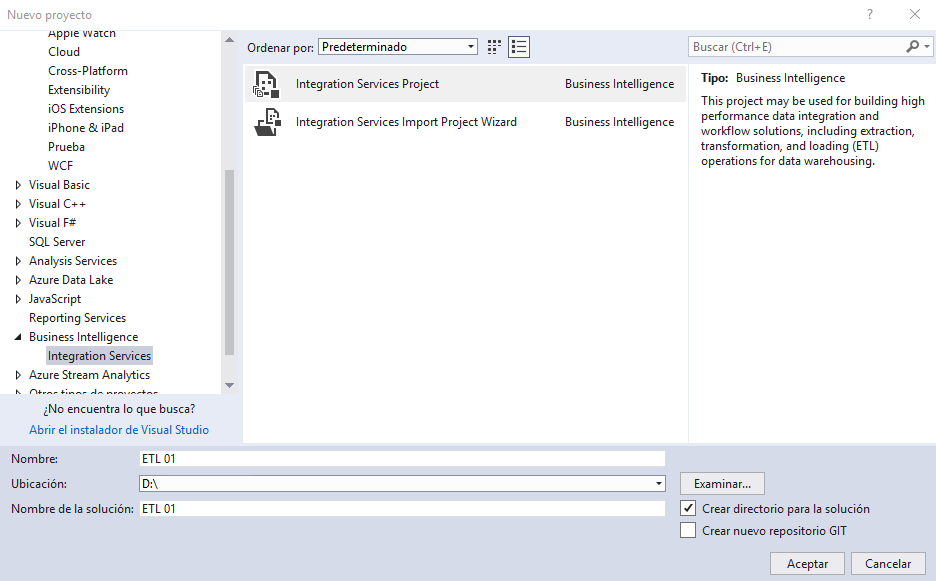
\includegraphics[width=11cm]{./Imagenes/img13}
	\end{center}	

2. En al ventana nueva, sección Solución Explorer, Agrego el paquete generado antes\\
	\begin{center}
	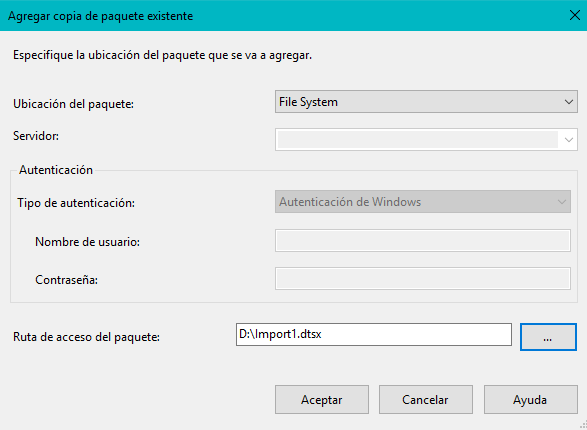
\includegraphics[width=11cm]{./Imagenes/img14}
	\end{center}	
	\begin{center}
	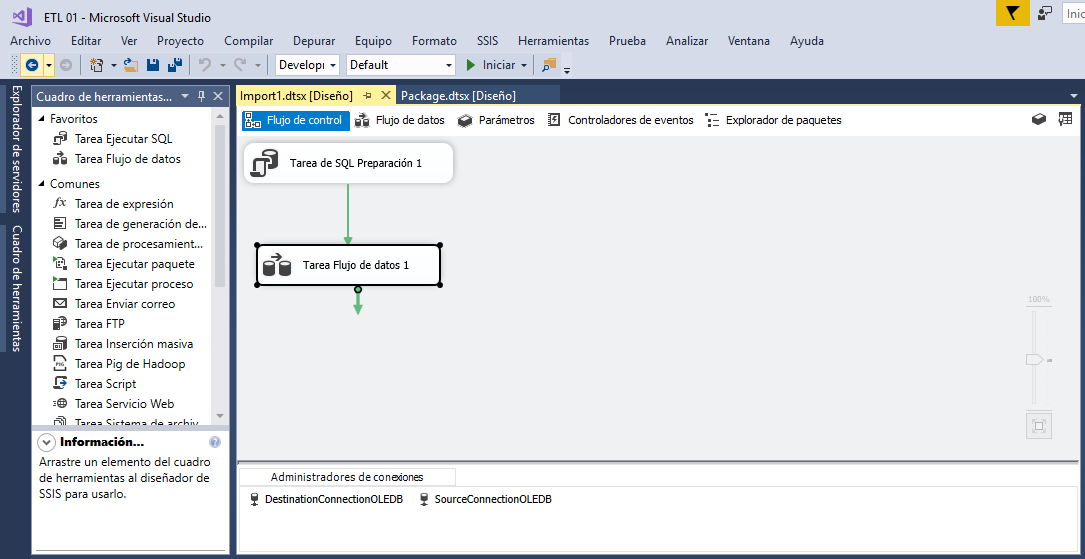
\includegraphics[width=11cm]{./Imagenes/img15}
	\end{center}	
	\begin{center}
	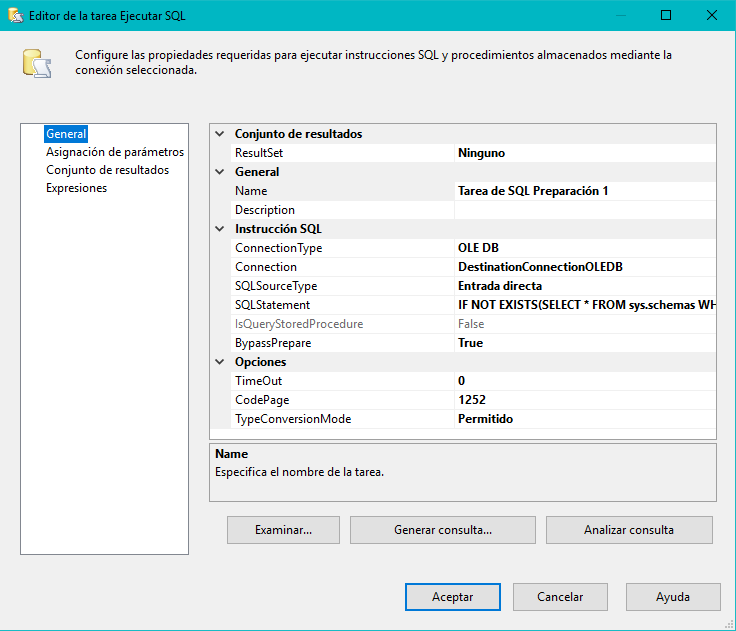
\includegraphics[width=11cm]{./Imagenes/img16}
	\end{center}	

3. En la siguiente ventana mostramos el paquete que se ha importado.\\
	\begin{center}
	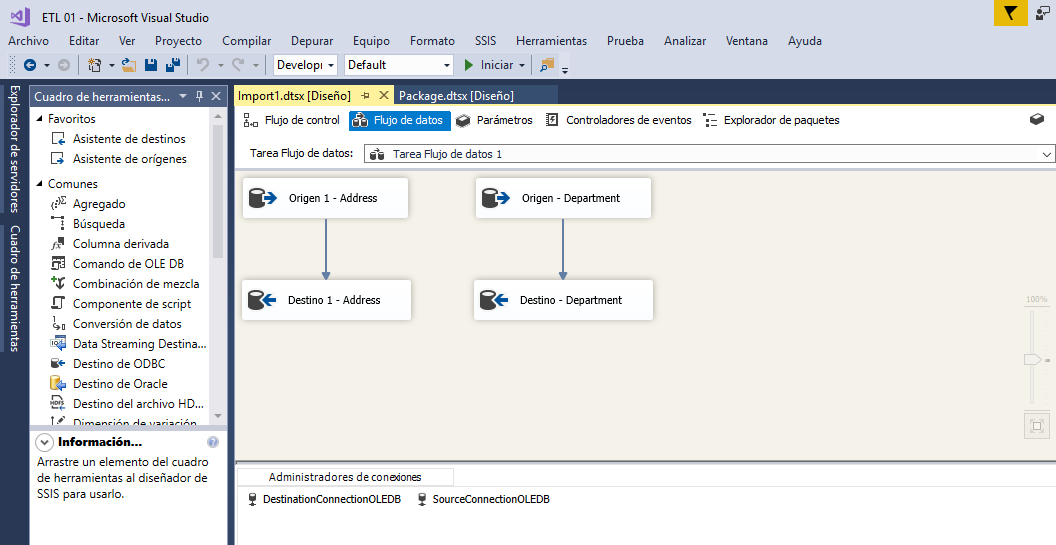
\includegraphics[width=11cm]{./Imagenes/img17}
	\end{center}	
	\begin{center}
	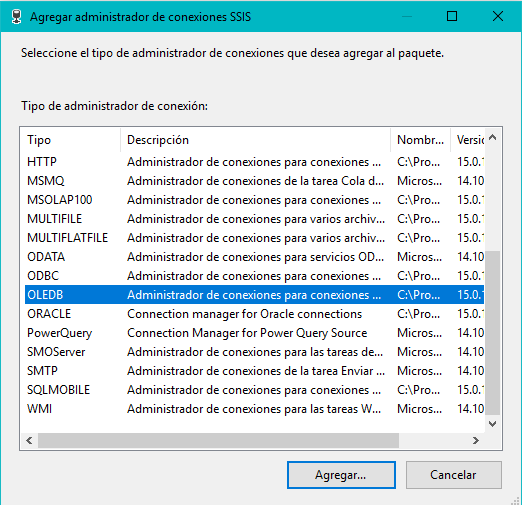
\includegraphics[width=11cm]{./Imagenes/img18}
	\end{center}	

4. En la siguiente ventana mostramos el paquete que se ha importado.\\
	\begin{center}
	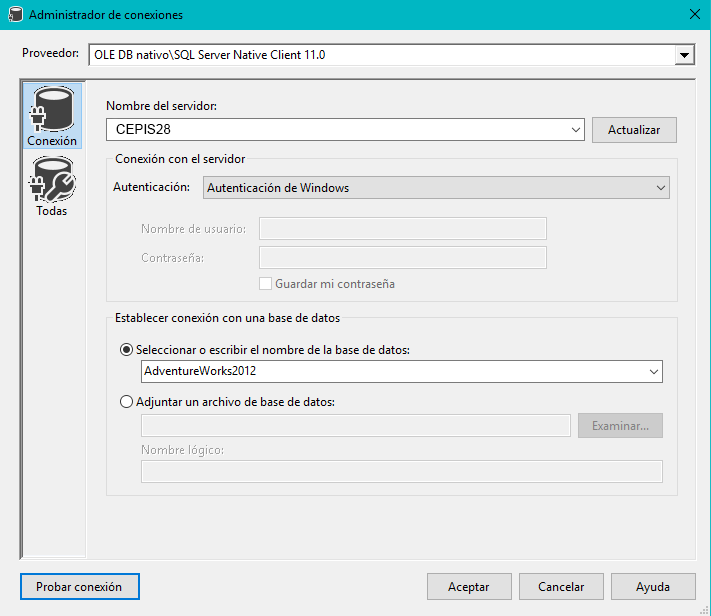
\includegraphics[width=11cm]{./Imagenes/img19}
	\end{center}	
	\begin{center}
	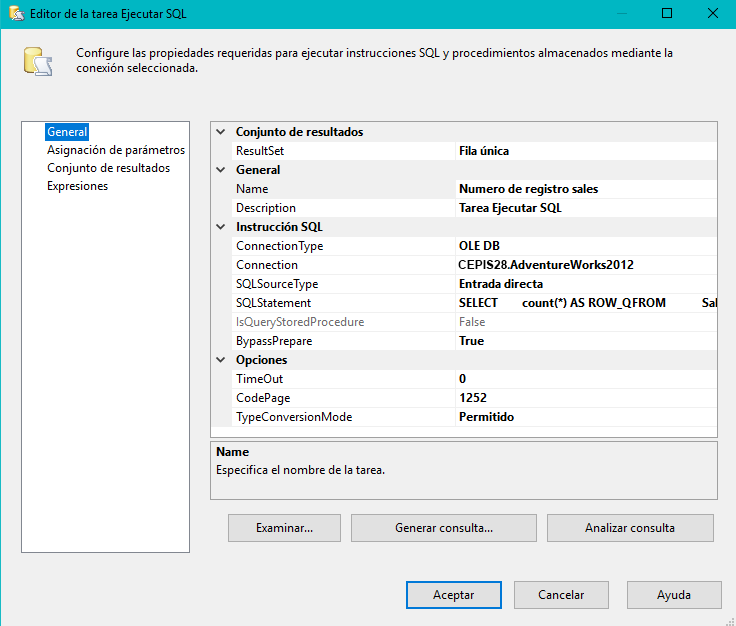
\includegraphics[width=11cm]{./Imagenes/img20}
	\end{center}	
	\begin{center}

5. Editamos el componente Scrtipt Task Editor.\\
	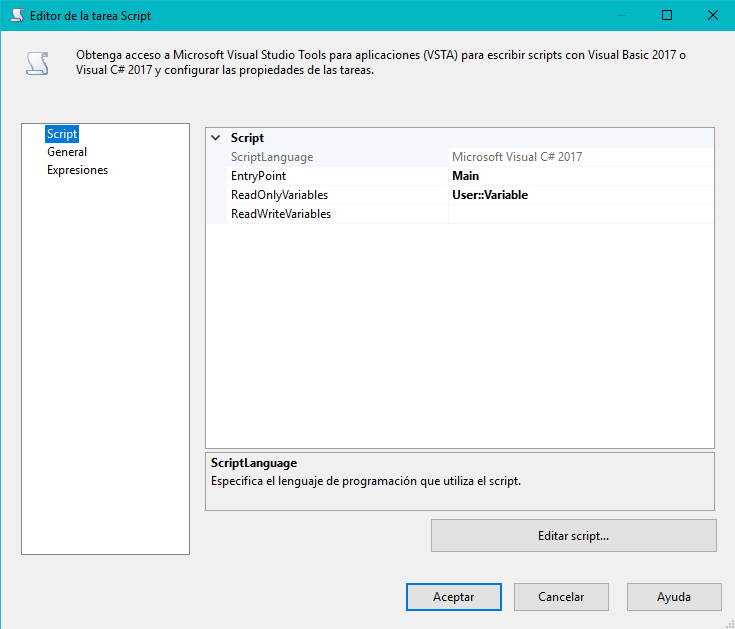
\includegraphics[width=11cm]{./Imagenes/img21}
	\end{center}	
	\begin{center}
	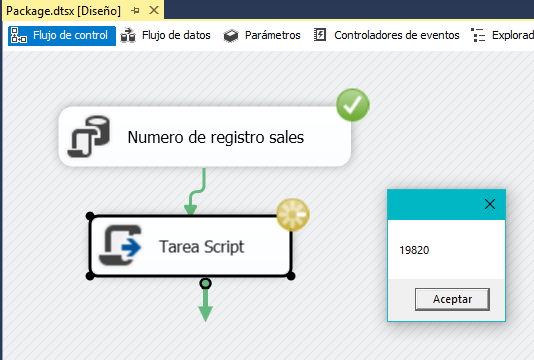
\includegraphics[width=11cm]{./Imagenes/img22}
	\end{center}	
	\begin{center}
	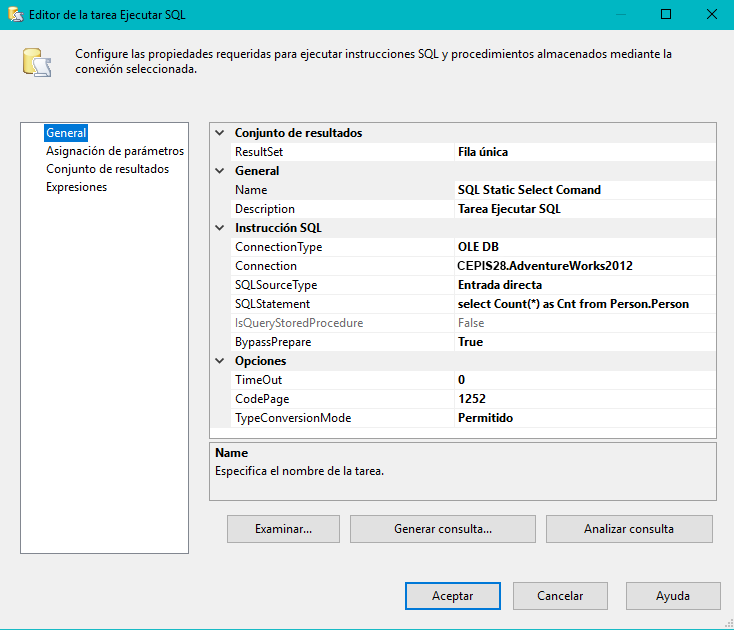
\includegraphics[width=11cm]{./Imagenes/img23}
	\end{center}	
	\begin{center}
	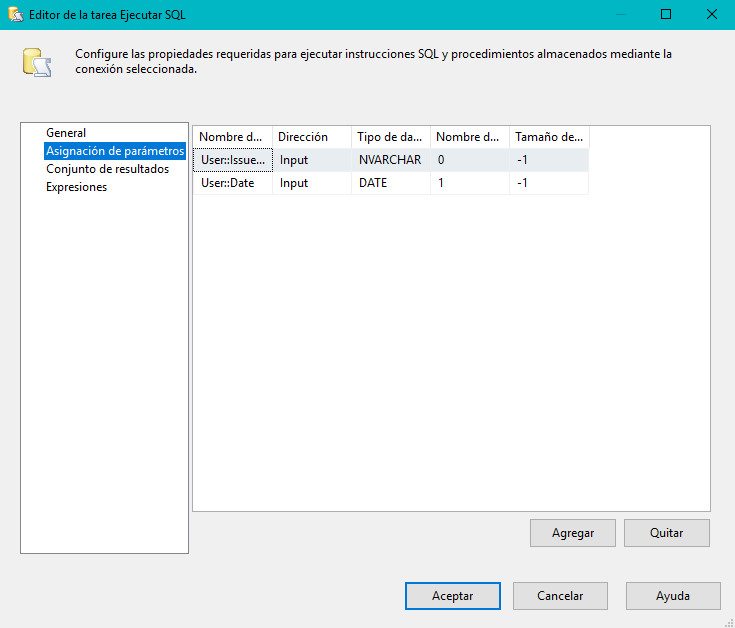
\includegraphics[width=11cm]{./Imagenes/img24}
	\end{center}	
	\begin{center}
	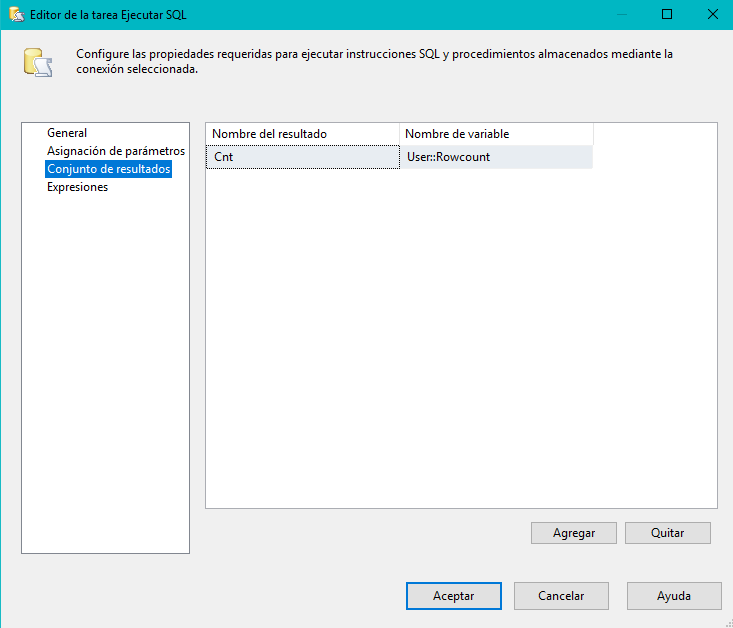
\includegraphics[width=11cm]{./Imagenes/img25}
	\end{center}	
	\begin{center}
	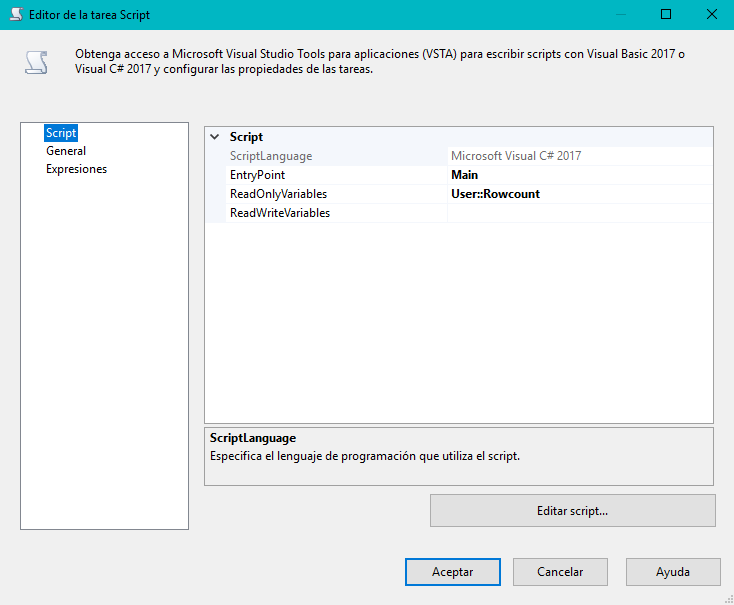
\includegraphics[width=11cm]{./Imagenes/img26}
	\end{center}	
	\begin{center}

6. Guardamos y los ejecutamos.\\
	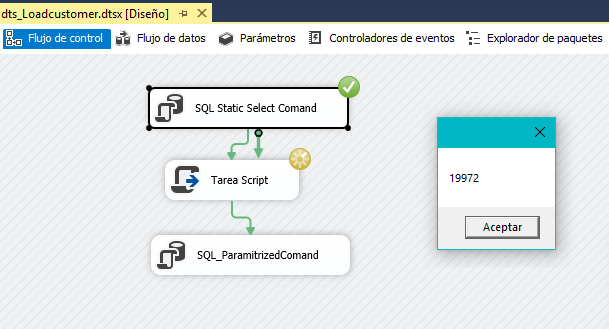
\includegraphics[width=11cm]{./Imagenes/img27}
	\end{center}	